\subsubsection{Overview}
The Save-Load system is the backbone of Computron. It is responsible for serializing and deserializing all the relevant player data needed to reconstruct play sessions. The system currently supports up to three player save slots to store game data. This restriction is an artificial one, as we only chose to allow the UI of the main menu to address three slots. The underlying mechanisms of the system can handle arbitrarily many save slots, as long as the player is given an interface to select them. An overview is provided by \ref{fig:saveload_system_diagram}.

\begin{figure}[!hb]
    \caption{Save-Load System Overview}
    \label{fig:saveload_system_diagram}
    \centering
    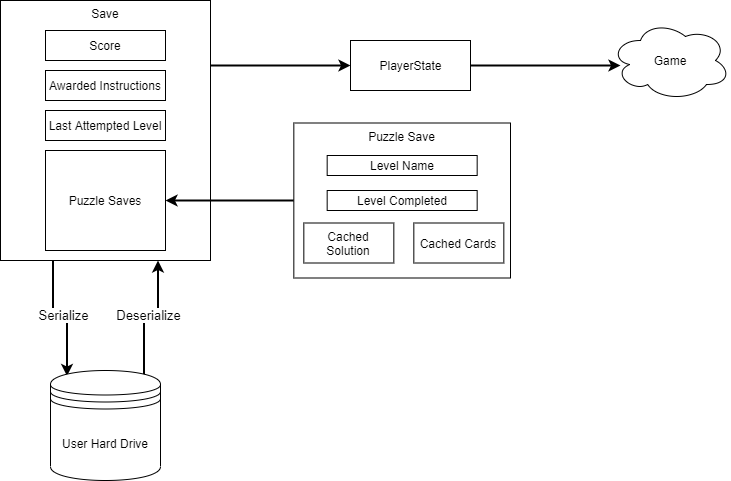
\includegraphics[width=\textwidth]{Diagrams/SaveLoad.png}
\end{figure}

As hinted to above, the only place in which the player actively interacts with the Save-Load system is at game startup. After hitting play, the player will be presented with a choice of three save slots, and the necessary UI to create, delete, or select a save in any of the three slots. 

\subsubsection{Data}
In this section you will find an enumeration of all the information required to restore user play sessions. Due to how this information is generated and captured, changes to the game's level layout can corrupt these save files and cause unexpected behavior in the level selection scene and puzzle scenes. It is highly recommended that developers clear outdated save files when adding, removing, or otherwise altering levels.

The top-level save object is simply called a Save. Below is an enumeration of the data captured in a save:
\begin{itemize}
    \item Player Score
    \item Awarded Instructions
    \item Last Attempted Level
    \item A collection of puzzle-specific saves for each puzzle the player has attempted
\end{itemize}

Top-level Saves defer the responsibility of tracking per-puzzle player data to a specialized serializable object cleverly know as a Puzzle Save. Puzzle Saves are generated and maintained on a per-level basis. When a player visits a level for the first time, a new entry is added to their save file for that level. This entry includes the following information:
\begin{itemize}
    \item The level's name
    \item Whether the level has been completed
    \item A list of what instructions the player left in the solution window
    \item A list of what cards the player left in the play area
    \item Which challenge stars the player has earned
\end{itemize}

\subsubsection{Scene Traversal}
After all this data is collected, and loaded (from either a binary or JSON save file) it is transferred to a PlayerState GameObject which travels between all scenes. This PlayerState object provides an interface for level generation systems read and write from player session data to configure the scenes and report significant game events.